\documentclass{beamer}
\usetheme[progressbar=foot, numbering=counter, block=fill]{metropolis}

\AtBeginSection[]
{
  \begin{frame}<beamer>
    \frametitle{Table of Contents}
    \tableofcontents[currentsection]
  \end{frame}
}

\title{Self-regulation and mathematics learning in the college classroom}
\date{September 18, 2018}
\author{Jenny Lee}
\institute{Harvey Mudd College\\Advisor: Dagan Karp}
\begin{document}
\maketitle
\begin{frame}{Recap \& Overview}
  \begin{itemize}
    \item Motivation
    \item Self-regulation in the context of college mathematics
    \item Self-paced assessment in the setting of Math 40
  \end{itemize}
\end{frame}
\begin{frame}{Motivation}
  \begin{center}
    \textit{``Individual differences'' in learners is a fact that can be demonstrated in many ways. That our students {\only<2> {\color{blue}}{vary in many ways}} can never be forgotten ... Our basic task in education is to find strategies which will take individual differences into consideration but which will do so in such a way as to {\only<3> {\color{blue}} promote the fullest development of the individual}.}
  \end{center}
  \hfill- Benjamin Bloom
\end{frame}
\begin{frame}{Status quo - Lecture based}
  \begin{itemize}
    \item Faculty to student ratio $\approx 1:20$
    \item Generalized instruction, individualized assessment
    \item Common end goal
  \end{itemize}
\end{frame}
\begin{frame}{Status quo - Lecture based}
  \centering
    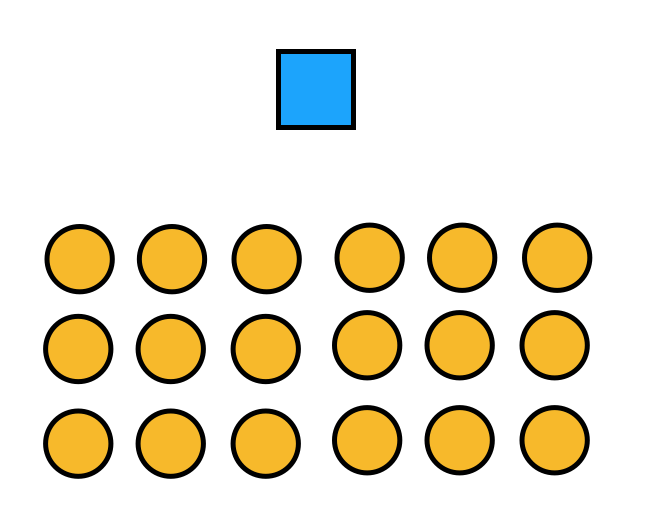
\includegraphics[scale=0.5]{lecturestyle1}
\end{frame}
\begin{frame}{Status quo - Lecture based}
  \centering
    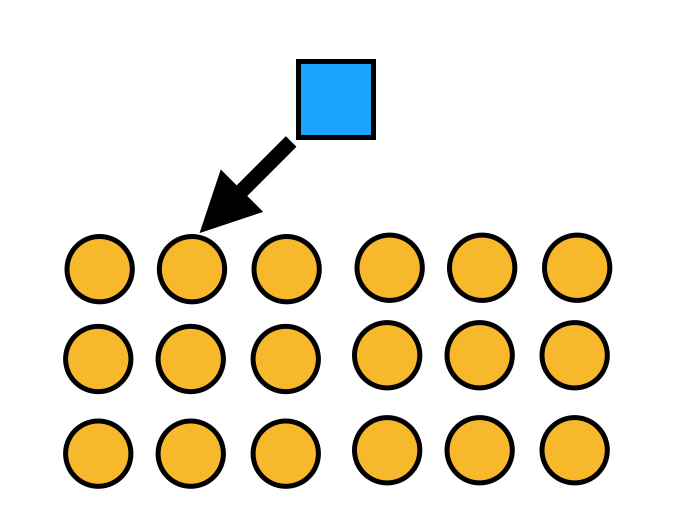
\includegraphics[scale=0.5]{lecturestyle3}
\end{frame}
\begin{frame}{Status quo - Lecture based}
  \centering
    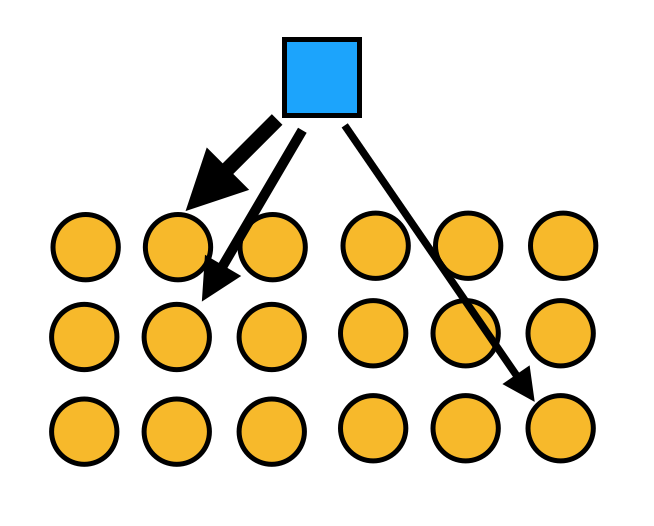
\includegraphics[scale=0.5]{lecturestyle2}\\
    \pause No arrow backwards.
\end{frame}
\begin{frame}
  How do we fix it?
\end{frame}
\begin{frame}
  Self-efficacy.\pause
  \begin{itemize}
    \item Feeling that one can succeed.
  \end{itemize}
\end{frame}
\begin{frame}{Self-regulation}
  Definition:
  \begin{center}
    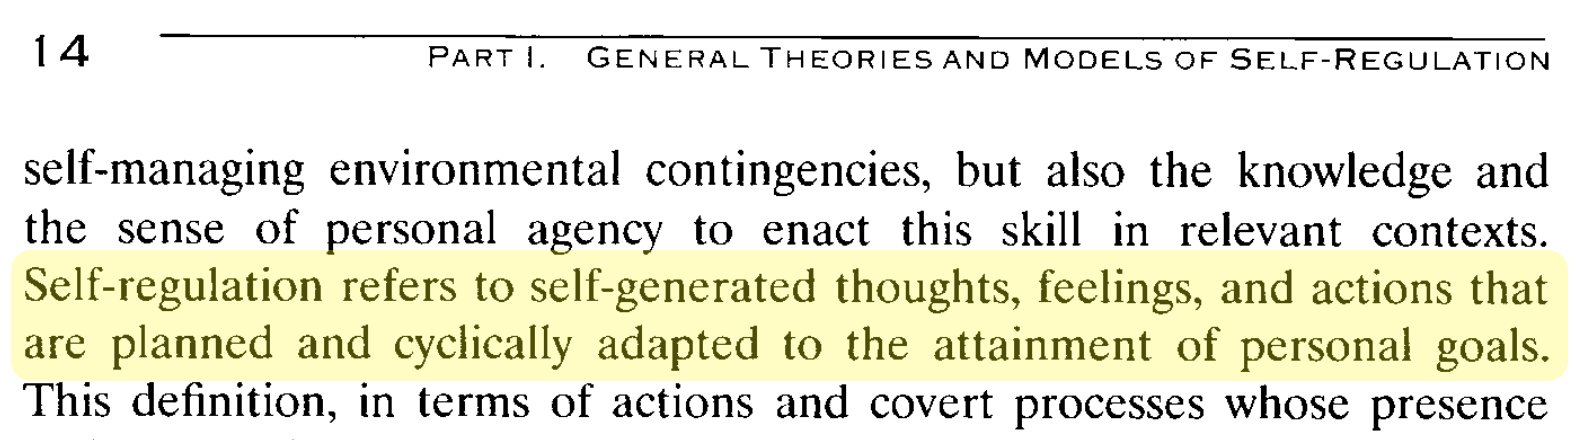
\includegraphics[scale=0.4]{selfregdef}
  \end{center}
  \hfill \begin{minipage}[]{7cm}
      \emph{\tiny Zeidner, M., Pintrich, P. R., \& Boekaerts, M. (2005). Handbook of Self-Regulation. Burlington, MA: Academic Press.}
\end{minipage}
\end{frame}
\begin{frame}{A form of self-regulation: self-assessment}
  \begin{itemize}
    \item Qualitative or quantitative evaluation
    \item Metacognitive exercises
    \item Goal: boost self-efficacy, shift locus of power
  \end{itemize}
\end{frame}
\begin{frame}{Various types of self-assessment}
  \begin{itemize}
    \item Self-instruction
    \begin{itemize}
      \item ex. Flipped classrooms, inquiry-based learning
    \end{itemize}
    \item Self-monitoring
    \begin{itemize}
      \item Immediate feedback via checklist
    \end{itemize}
  \end{itemize}
\end{frame}
\begin{frame}{Self-paced assessment}
  \begin{itemize}
    \item What is it?\pause
    \item Considerations:
    \begin{itemize}
      \item subject, type of class, size of class
      \item existence of an honor code, TA's, other resources
      \item amount of instructor effort
      \item assessment
    \end{itemize}
  \end{itemize}
\end{frame}
\begin{frame}{Case study: Math 40}
  \begin{itemize}
    \item Ideal (school, size, subject)
    \item Implementation
    \begin{itemize}
      \item Students in section A - regular midterm/exam
      \item Students in section B - multiple take-home quizzes with multiple retries without penalty
    \end{itemize}
  \end{itemize}
\end{frame}
\begin{frame}{Results from the case study}
  \begin{itemize}
    \item ``No negatives'' == equally effective
    \item Positive student experience
  \end{itemize}
\end{frame}
\end{document}
